\documentclass[addpoints,11pt]{exam}

\usepackage{alltt}
\usepackage[margin=1in]{geometry}   % set up margins
\usepackage[T1]{fontenc}
\usepackage[usenames,dvipsnames]{xcolor}
\usepackage{enumerate}              % fancy enumerate
\usepackage{amsmath}                % used for \eqref{} in this document
\usepackage{amsthm}
\theoremstyle{definition}
\newtheorem{exmp}{Example}[section]
\usepackage{verbatim}               % useful for \begin{comment} and \end{comment}
\usepackage{eurosym}                % used for euro symbol
\usepackage{caption} 
\usepackage{graphicx}
\graphicspath{{Figures/}}
\usepackage{subcaption}
\usepackage{color}
\usepackage{float}
\usepackage{amssymb}
\usepackage{sgamevar}
\usepackage{sgame}
\usepackage[colorlinks=true]{hyperref}
\hypersetup{colorlinks=true, citecolor=ForestGreen, linkcolor=BlueViolet, urlcolor=Magenta}

%Solutions or nah (blank next two lines out for no solutions, unblank #3)
%\printanswers
%\newcommand{\dd}[1]{\par {\textbf{\textcolor{red}{#1}}}}
\newcommand{\dd}[1]{}  


\setlength\parindent{0pt}
\unframedsolutions
\SolutionEmphasis{\color{red}}
\CorrectChoiceEmphasis{\color{red}}
\renewcommand{\choicelabel}{(\alph{choice})}
\newcommand{\blank}[0]{\underline{\hspace{3cm}}}
\pointformat{\bfseries[\thepoints]}
\pointpoints{pt}{pts}
\pointsinrightmargin




\begin{document}


\title{\textbf{Exam 2} \dd{Solutions} \\ \vspace{2 mm} {\large ECON 101}}
\author{Summer I 2015}
\date{}
\maketitle

\makebox[\textwidth]{Name:\enspace\hrulefill}
\\

\makebox[\textwidth]{ONYEN:\enspace\hrulefill}
\\

\makebox[\textwidth]{PID:\enspace\hrulefill}
\\

\makebox[\textwidth]{Honor Code Signature:\enspace\hrulefill}

\begin{center}
	\fbox{\fbox{\parbox{5.5in}{\centering
				This exam consists of 30 multiple choice questions and 3 short answer questions. Multiple choice questions should be bubbled in on a scantron. Extra paper for scratch work is attached. The total number of points available on this exam is \textbf{100}.}}}
\end{center}

\section*{Multiple Choice [2 pts each]}

Choose the option that best answers the question given.

\begin{questions}
	
\question Natalie just graduated from college. In order to devote all her efforts towards her education, she didn't hold a job while in school. Now, she is going to cruise around the country on her motorcycle for awhile before she starts looking for work. As a result, the unemployment rate

\begin{choices}
		\choice increases, and the labor-force participation rate increases.
		\CorrectChoice is unaffected, and the labor-force participation rate is unaffected.
		\choice increases, and the labor-force participation rate decreases. 
		\choice increases, and the labor-force participation rate is unaffected.
\end{choices}

	
\question Acme, LLC is considering purchasing a new factory. If the interest rate falls, then the present value of the returns from the factory will \blank, and the company will be \blank likely to build the factory.

		\begin{choices}
			\choice increase; less
			\choice decrease; more
			\CorrectChoice increase; more
			\choice decrease; less
		\end{choices}
		
\newpage

	\question For a firm in a monopolistically competitive market, which of the following accurately describes the relationship between the price, average total cost, and marginal cost in the long run?
	
	\begin{choices}
			\choice $P = ATC = MC$
			\choice $P > ATC = MC$
			\CorrectChoice $P = ATC > MC$
			\choice $P > ATC > MC$
	\end{choices}

	
	\question Which of the following is NOT a kind of institution encouraging investment and the efficient organization of the factors of production?
	
	
	\begin{choices}
			\choice A dependable legal system
			\choice Political stability
			\choice An honest government
			\CorrectChoice Social safety nets
	\end{choices}
	


\question Suppose a country is currently at its steady state. If the country decides to permanently decrease its savings rate, which of the following must be true?

	\begin{enumerate}[i.]
		\item Consumption will immediately increase, and the new steady state consumption level will be greater than the old steady state consumption level.
		\item Investment will immediately decrease, and the new steady state investment level will be less than the old steady state investment level.
		\item The new steady state level of capital will be less than the old steady state level of capital, and the new steady state level of output will be less than the old steady state level of output.
	\end{enumerate}
	
\begin{choices}
	\choice i and ii
	\choice i and iii
	\CorrectChoice ii and iii
	\choice i, ii, and iii
\end{choices}


\question Country $X$ and country $Y$ both have the same production function, $f(k)=1.5\sqrt{k}$. Moreover, the current level of capital per worker in each country is $k_0 = 400$. In country $X$, output per worker is growing, while in country $Y$ it is falling. According to the Solow Model, \textit{ceteris paribus}, which of the following could account for this difference?
	
	\begin{choices}
		\CorrectChoice The savings rate in country $X$ is greater than that in country $Y$.
		\choice The population growth rate in country $X$ is greater than that in country $Y$.
		\choice Capital depreciates faster in country $X$ than in country $Y$.
		\choice Any of the above could account for this difference.
		\choice None of the above could account for this difference.
	\end{choices}
	
\newpage

\question A bag of sugar is sold to Coca Cola for \$0.50, which uses this sugar to make Sprite that is sold to consumers for \$1.25. Another bag of of sugar is sold to Food Lion for \$1.25, where it is sold to consumers for \$2.75. Together, these transactions have what effect on GDP?


\begin{choices}
		\choice Increase GDP by \$1.75
		\CorrectChoice Increase GDP by \$4.00
		\choice Increase GDP by \$5.75
		\choice Increase GDP by \$3.00
\end{choices}

	
\question Consider the simultaneous move game between Jim and Bob shown below, where the first number in each block is the payoff to Bob and the second is the payoff to Jim.

\renewcommand{\gamestretch}{1.5}
\sgcolsep=25pt
\begin{figure}[htb]\hspace*{\fill}%
	\begin{game}{2}{2}[Bob][Jim] 
		&  Left & Right \\
		Top & 2, 4 & $x$, 2 \\
		Bottom & 1, $y$ & 2, 3 \\
	\end{game} 
	\hspace*{\fill}%
\end{figure}

If ``Top'' is the dominant strategy for Bob and ``Left'' is the 	dominant strategy for Jim, then possible values of $x$ and $y$ are

		\begin{choices}
		\choice $x=1$ and $y=2$.
		\choice $x=1$ and $y=4$.
		\choice $x=3$ and $y=2$.
		\CorrectChoice $x=3$ and $y=4$.
		\end{choices}

	
\question Suppose a firm sells 25 units at a price of \$10. Calculate its marginal revenue per unit of output if it sells 5 more units of output when it reduces its price to \$9. Is this firm in a  competitive market or non-competitive market?
		
		\begin{choices}
				\choice \$20; non-competitive
				\CorrectChoice \$4; non-competitive
				\choice \$270; non-competitive
				\choice \$2.50; competitive
				\choice None of the above.
		\end{choices}
	
\uplevel{Use Figure \ref{MC10}, which represents the environment faced by a monopoly, for questions \ref{q10}-\ref{q11}.}
	
	\begin{figure}[H]
		\centering
		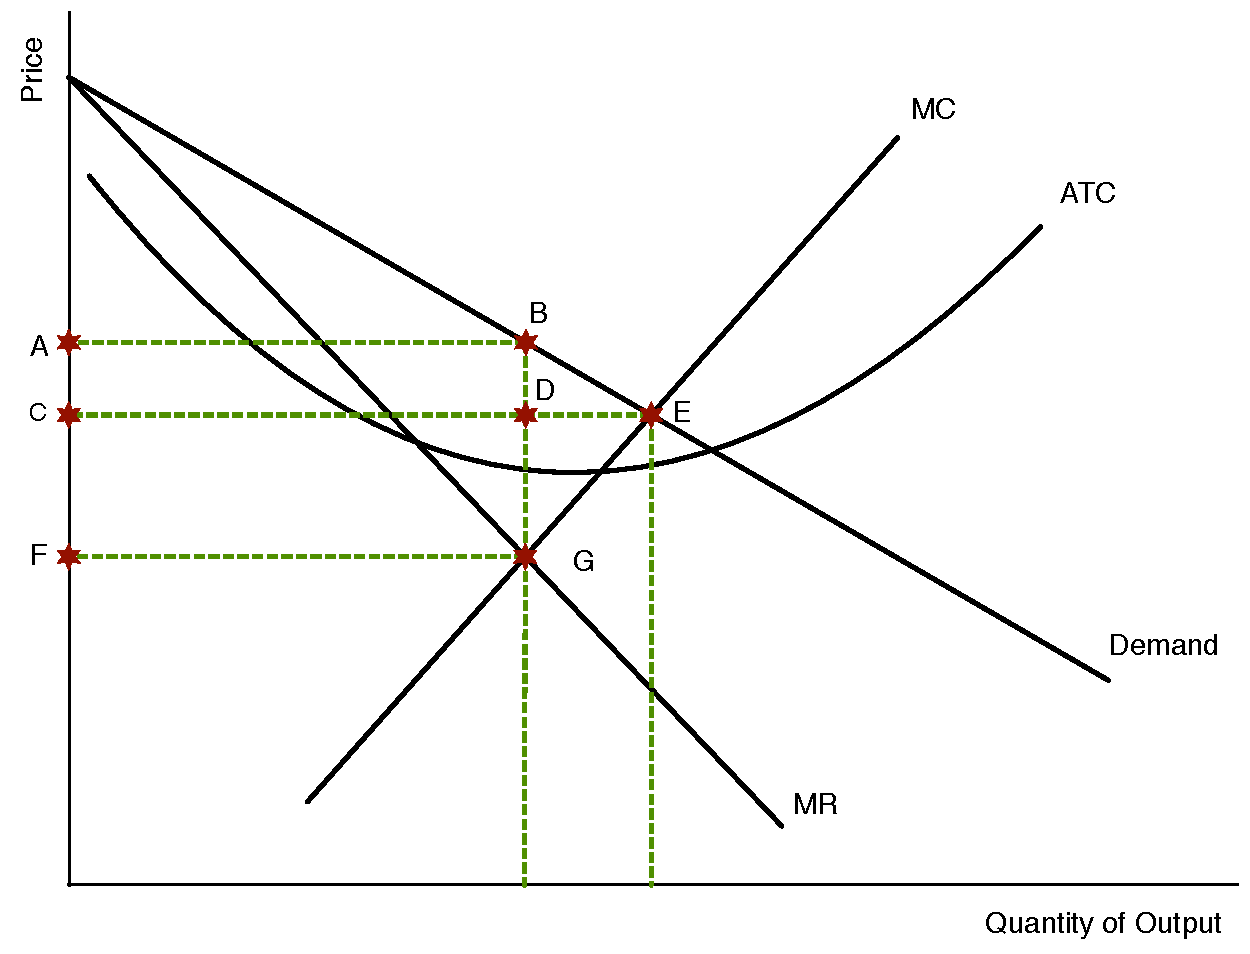
\includegraphics[scale=.4]{Exam2_MC10.pdf}
		\caption{Monopolist Environment}
		\label{MC10}
	\end{figure}

	\question \label{q10} Which of the following represents the lost trade that is responsible for the deadweight loss?
	
	
	\begin{choices}
		\choice Distance ab
		\choice Distance ce
		\CorrectChoice Distance de
		\choice Distance cd
	\end{choices}
	
	
	\question \label{q11} Which of the following areas represents the deadweight loss due to monopoly pricing?
	
	\begin{choices}
			\CorrectChoice Triangle bge
			\choice Triangle bde
			\choice Rectangle acdb
			\choice Rectangle cfgd
	\end{choices}
	

	
\question Jonathan takes \$500 of currency from her wallet and deposits it in a checking account. If the bank adds the entire \$500 to reserves, the money supply \underline{\hspace{3cm}}, but if the bank lends out some of the \$500, the money supply \underline{\hspace{3cm}}.
		
		
		\begin{choices}
				\choice increases; increases even more
				\choice increases; increases by less
				\CorrectChoice is unchanged; increases
				\choice decreases; decreases by less
		\end{choices}
		

	
	\question The actual unemployment rate varies around the 
	
	\begin{choices}
			\choice frictional unemployment rate.
			\choice structural unemployment rate.
			\choice cyclical unemployment rate. 
			\CorrectChoice natural employment rate.
	\end{choices}

	
	\question Intel and AMD each decide to either invest heavily in R\&D (``High R\&D'') or to not (``Low R\&D''). Their decisions affect both their profits and those of the other company. Assume that there is perfect information so that each knows the payoffs of the other given the strategies chosen by each. Their profits are summarized in the game table below, where the first number in each block is AMD's profit and the second number is Intel's profit.
	
	\renewcommand{\gamestretch}{1.5}
	\sgcolsep=25pt
	\begin{figure}[htb]\hspace*{\fill}%
		\begin{game}{2}{2}[AMD][Intel] 
			&  High R\&D & Low R\&D \\
			High R\&D & \$15,000, \$20,000 & \$18,000, \$15,000 \\
			Low R\&D & \$16,000, \$18,000 & \$16,000, \$15,000\\
		\end{game} 
		\hspace*{\fill}%
	\end{figure}
	
	If this game was played once and Intel and AMD are both rational, what would be the outcome?
	
	\begin{choices}
			\CorrectChoice Intel would invest heavily in R\&D and AMD would not.
			\choice Both Intel and AMD would invest heavily in R\&D.
			\choice AMD would invest heavily in R\&D and Intel would not.
			\choice Both Intel and AMD would choose to not invest heavily in R\&D.
	\end{choices}

	
	\question Savings is 
	

	
	\begin{choices}
		\choice the purchase of new capital goods.
		\choice the purchase of new consumption goods.
		\choice income that is not spent on capital goods.
		\CorrectChoice income that is not spent on consumption goods. 
	\end{choices}	
	

	
	\question Which of the following would be considered an increase in human capital?
	
		\begin{choices}
			\CorrectChoice An increase in the training of heart disease researchers.
			\choice An increase in the use of heart disease centers.
			\choice The discovery of a cure for broken hearts.
			\choice An increase in the number of heart disease researchers.
		\end{choices}
		

		
	\question Assume an economy experienced a positive rate of inflation between 2003 and 2004 and again between 2004 and 2005. However, the inflation rate was lower between 2004 and 2005 than it was between 2003 and 2004. Which of the following scenarios is consistent with this assumption?


	
	\begin{choices}
		\choice The CPI was 100 in 2003, 110 in 2004, and 105 in 2005.
		\CorrectChoice The CPI was 100 in 2003, 120 in 2004, and 135 in 2005.
		\choice The CPI was 110 in 2003, 106 in 2004, and 100 in 2005.
		\choice All of the above are correct.
	\end{choices}
	
	
	\question  If the Fed wanted to increase the money supply, it could
	
		
		\begin{choices}
			\CorrectChoice purchase government bonds.
			\choice increase the required reserve ratio.
			\choice increase the discount rate.
			\choice increase the interest rate on reserves.
		\end{choices}
	
	\question A family in Ireland purchases leather loafers from a shoe maker in Italy. As a result of this transaction, GDP in Ireland \blank and GDP in Italy \blank. 
	
	\begin{choices}
		\choice increases; remains unchanged
		\choice remains unchanged; decreases
		\choice decreases; increases
		\CorrectChoice remains unchanged; increases
		\choice None of the above
	\end{choices}
	

		
	\question Firms in monopolistically competitive markets are similar to monopolies in that they both \blank and are similar to firms in perfectly competitive markets in that they both \blank.
	

		\begin{choices}
				\choice make positive profits in the short and long run; produce at the efficient scale in the long run.
				\CorrectChoice charge a price above the marginal cost; can freely enter and exit the market.
				\choice are price makers; produce at the efficient quantity.
				\choice are in markets with barriers to entry; make zero economic profit in the long run.
		\end{choices}	

	
	\question Suppose an economy contains 2,000 \$1 bills. If people initially deposit half their currency as demand deposits while banks maintain 100\% reserves, the maximum quantity of money would be \blank. If, however, people initially deposit half their currency as demand deposits while banks maintain 10\% reserves, the maximum quantity of money in the economy would be \blank.
	
	\begin{choices}
		\choice \$2,000; \$10,000
		\choice \$1,000; \$10,000
		\choice \$1,000; \$11,000
		\CorrectChoice \$2,000; \$11,000
	\end{choices}
	

\question Suppose the real GDP in Slovenia in 1950 was \$50,000. If by 1977, the real GDP was \$200,000, what was the approximate \textit{annual} growth rate in the country from 1950 to 1977?


\begin{choices}
		\choice 2.6\%
		\choice 300\%
		\choice 4.0\%
		\CorrectChoice 5.2\%
\end{choices}


	
\question Table \ref{MC23} shows the prices and quantities produced of the only two goods in Uzbeki-beki-beki-Stan-Stan, grapes and olives, for the years 2000 -- 2002.

\begin{table}[H]
	\caption{Grapes and Olives in UZN}
	\centering
	\begin{tabular}{c|c|c|c|c}
		Year & Grapes Produced & Price of Grapes & Olives Produced & Price of Olives \\
		\hline
		2000 & 20 & \$2.10 & 4 & \$4.10\\
		2001 & 19 & \$2.25 & 6 & \$4.15\\
		2002 & 22 & \$2.20 & 7 & \$4.15\\
	\end{tabular} 
	\label{MC23}
\end{table}

Using 2001 as the base year, the real GDP in 2000 is \blank. Additionally, the inflation rate in 2001 was \blank.


\begin{choices}
	\choice \$61.60; 3.2\%
	\choice \$58.4; 5.5\%
	\CorrectChoice \$61.60; 5.5\%
	\choice \$58.4; 3.2\%
\end{choices}


	
	\question One of the widely-acknowledged problems with the consumer price index (CPI) as a measure of the cost of living is that the CPI
	
	\begin{choices}
		\choice fails to account for consumer spending on housing.
		\choice accounts only for consumer spending on food, clothing, and energy.
		\choice fails to account for the fact that consumers spend larger percentages of their incomes on some goods and smaller percentages of their incomes on other goods.
		\CorrectChoice fails to account for the introduction of new goods.
	\end{choices}
	
	
	\question Bandidos and Carrburritos are the only taco sellers in Chapel Hill. They face the environment outlined in Table \ref{MC24}. 
	
	\begin{table}[H]
		\caption{Demand Schedule and Costs for Tacos in CH}
		\centering
		\begin{tabular}{c|c|c}
			Price & Quantity Demanded & Average Total Cost \\
			\hline
			\$10 & 200 & \$4\\
			\$9 & 300 & \$4\\
			\$8 & 400 & \$4 \\
			\$7 & 500 & \$4 \\
			\$6 & 600 & \$4 \\
		\end{tabular} 
		\label{MC24}
	\end{table}
	
	The two firms currently have an agreement where they produce 400 tacos in total and split production evenly. If Bandidos were to break this agreement and increased their taco production by 100 tacos while Carrburritos stuck to the original agreement, the profit realized by Bandidos would now be \underline{\hspace{3cm}} and the profit realized by Carrburritos would be \blank.
	
	
	\begin{choices}
		\CorrectChoice \$900; \$600
		\choice \$750; \$750
		\choice \$900; \$700
		\choice \$800; \$800
	\end{choices} 
	

	\question A monopolistically competitive firm will decrease its production if
	
	\begin{choices}
		\choice marginal revenue is less than average total cost.
		\choice price is less than marginal cost.
		\CorrectChoice marginal revenue is less than marginal cost.
		\choice price is less than average total cost.
	\end{choices}	

\newpage
	
	\question Suppose the CPI in 2001 using 1982 as the base year was 262. The average salary of accounting majors in 1982 was \$45,500, while in 2001 it was \$74,000. Given this information, we can say that accounting majors in 2001 were
	
	\begin{choices}
		\choice better off than accounting majors in 1982.
		\CorrectChoice worse off than accounting majors in 1982.
		\choice equally as well off as accounting majors in 1982.
		\choice Not enough information given.
	\end{choices}
	
	
	\question Figure \ref{MC27} shows the market for loanable funds. 
	
	
	\begin{figure}[H]
		\centering
		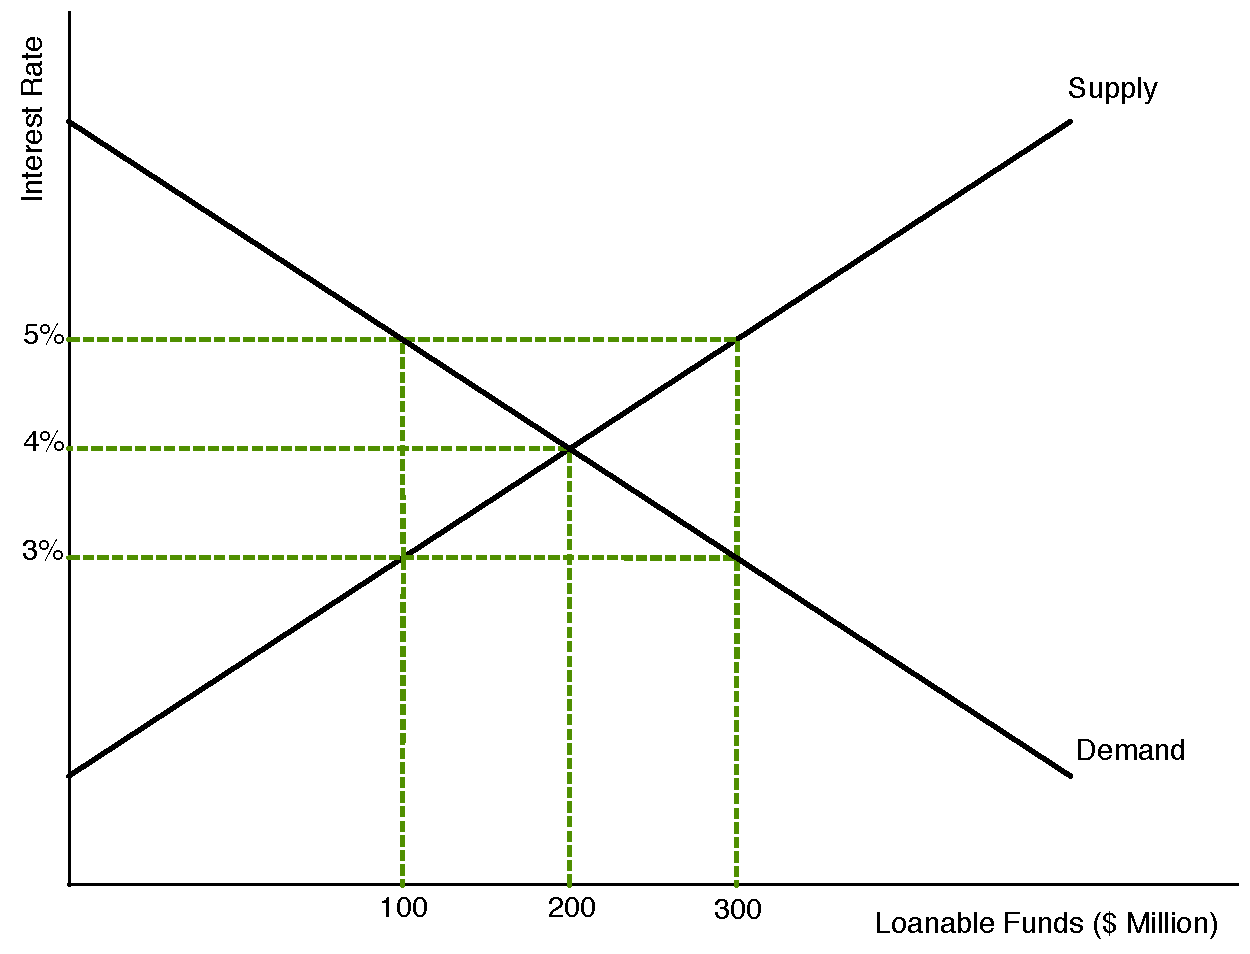
\includegraphics[scale=.4]{Exam2_MC27.pdf}
		\caption{Market for Loanable Funds}
		\label{MC27}
	\end{figure}
	
	If the interest rate in the market is 3\%, then 
	
	\begin{choices}
			\choice investment exceeds savings by \$300 million.
			\choice investment exceeds savings by \$200 million.
			\choice borrowing demands exceed savings by \$300 million.
			\CorrectChoice borrowing demands exceed savings by \$200 million.
	\end{choices}
	

	\question Consider Table \ref{MC28}, which shows the people in country $Y$ that are structurally unemployed, cyclically unemployed, and frictionally unemployed. 
	
	
	\begin{table}[H]
		\caption{Unemployment Statistics for Country $Y$}
		\centering
		\begin{tabular}{  c | c} 
			
			Type of Unemployment & Number Unemployed\\
			\hline
			Structural &  14 million\\
			Cyclical &  8 million\\
			Frictional & 10 million\\
		\end{tabular}
		\label{MC28}
	\end{table}
	
	
	Additionally, there are 300 million people employed and 350 million adults in the country. What is the \textit{natural} unemployment rate in country $Y$?
	
\newpage
	
	\begin{choices}
		\CorrectChoice 7.2\%
		\choice 8.0\%
		\choice 9.1\%
		\choice 9.6\%
	\end{choices}
	
	
	\question Figure \ref{MC30} shows the production function of Iceland, as well as their investment function and depreciation function.
	
	
	\begin{figure}[H]
		\centering
		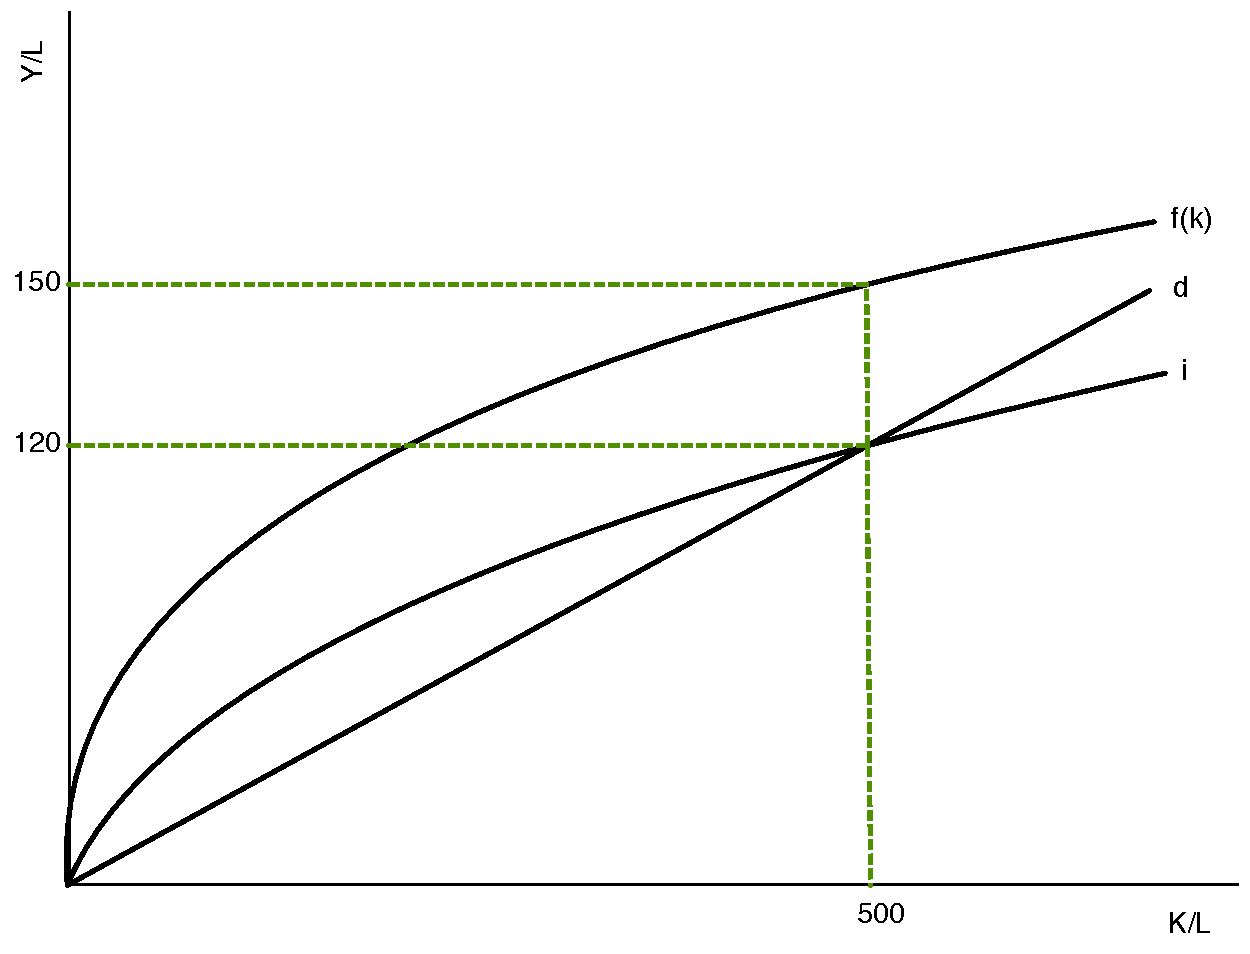
\includegraphics[scale=.4]{Exam2_MC30.pdf}
		\caption{Production in Iceland}
		\label{MC30}
	\end{figure}
	
	The amount of capital per worker that depreciates each period in the steady state is \underline{\hspace{3cm}} and the percent of output per worker that is consumed in the steady state is \underline{\hspace{3cm}}.
	
	
	\begin{choices}
			\choice 500; 80\%
			\CorrectChoice 120; 20\%
			\choice 500; 20\%
			\choice 120; 80\%
	\end{choices}
	
	
\end{questions}

\section*{Short Answer}

For this section, make sure to write legibly and box final answers. \textbf{Show your work!} This can be done within the section or \textit{clearly} labeled on the scratch paper provided.

\begin{questions}
	

\question Use the game matrix below to answer the questions that follow.

\renewcommand{\gamestretch}{1.5}
\sgcolsep=25pt
\begin{figure}[htb]\hspace*{\fill}%
	\begin{game}{3}{3}[Noah][Isabella] 
		&  Run & Walk & Crawl \\
		Run & 2, 1 & 4, 4 & 8, 2 \\
		Walk & 3, 0 & 1, 3 & 2, 2 \\
		Crawl & 3, 4 & 5, 5 & 4, 4 \\
	\end{game} 
	\hspace*{\fill}%
\end{figure}
	
\begin{parts}
	\part[3] Does Noah have a dominant strategy? If so, what is it? 
	\vspace{1cm}


	\part[3] Does Isabella have a dominant strategy? If so, what is it?
	\vspace{1cm}

	\part[4] If there are any, what are the Nash equilibrium in this game? Explain why.
	\vspace{1.5cm}

\end{parts}
	
\question Suppose a country has the production function $y=10\sqrt{k}$, a savings rate $s=20\%$, and capital depreciates at rate $\delta = 4\%$. The labor force is very elderly, and as a whole the country's workforce decreases 2\% every period.

\begin{parts}
	\part[4] What is the steady state level of capital and output in this country (in per worker terms)?
	\vspace{4cm}
	
	\part[4] What is the steady state level of investment and consumption in this country (in per worker terms)?
	\vspace{4cm}
	
	
	\part[4] Assume the country is at its steady state at $t=400$. At the start of $t=403$, the country decides to decrease the savings rate to $s_1 = 10\%$. What will be the growth rate of output per worker between $t=403$ and $t=404$? 
	\vspace{4cm}	

	\part[3] Draw the effect of this change in the savings rate on a well-labeled graph. You do not need to write the specific numbers down, but clearly show the steady state levels of capital, output, investment, and consumption before and after the change. 
	\vspace{4cm}
\end{parts}


\question Suppose the government borrows \$20 billion more next year than this year. Assume that the supply of loanable funds is made up of national savings.

\begin{parts}
\part[5] Use a supply and demand diagram to analyze this policy. What happens to the real interest rate? 
\vspace{3cm}

\part[4] What happens to private investment as a result? What is this change in private investment called? 
\vspace{2cm}

\part[3] How does the elasticity of the supply for loanable funds affect this change in private investment?
\vspace{2cm} 

\part[3] How does the elasticity of the demand for loanable funds affect this change in private investment? 
\vspace{2cm}

\end{parts}
 

\end{questions}


\hrulefill
\begin{center} 
	\textbf{END OF EXAM}
\end{center}

\newpage

\centering

\section*{SCRATCH SHEET}


\end{document}